\documentclass{article}
\usepackage[utf8]{inputenc}
\usepackage[portuguese]{babel}
\usepackage{hyperref}
\usepackage{float}
\usepackage{comment}
\usepackage{listings}
\usepackage{courier}
\usepackage{xcolor}
\usepackage{color}
\usepackage{calc}
\usepackage{enumerate}
\usepackage{todonotes}
\usepackage{graphicx,url}
\usepackage{float}
\usepackage{amsmath}
\usepackage{mathtools}

\title{Análise e Transformações de programas \\
\vspace{7.5pt} 
\textbf{Software Rejuvenation}}
\author{Walter Mendonça}
\date{2023} 

\definecolor{javared}{rgb}{0.6,0,0} % for strings
\definecolor{javagreen}{rgb}{0.25,0.5,0.35} % comments
\definecolor{javapurple}{rgb}{0.5,0,0.35} % keywords
\definecolor{javadocblue}{rgb}{0.25,0.35,0.75} % javadoc

\lstset{
  basicstyle=\footnotesize\tt,        % the size of the fonts that are used for the code
  breakatwhitespace=false,         % sets if automatic breaks should only happen at whitespace
  breaklines=true,                 % sets automatic line breaking
  captionpos=t,                    % sets the caption-position to bottom
  extendedchars=true,              % lets you use non-ASCII characters; for 8-bits encodings only, does not work with UTF-8
  frame=single,                    % adds a frame around the code
  language=Java,                 % the language of the code
  keywordstyle=\bf,
  showspaces=false,                % show spaces everywhere adding particular underscores; it overrides 'showstringspaces'
  showstringspaces=false,          % underline spaces within strings only
  showtabs=false,                  % show tabs within strings adding particular underscores
  tabsize=2,                       % sets default tabsize to 2 spaces
  keywordstyle=\color{javapurple}\bfseries,
  stringstyle=\color{javared},
  commentstyle=\color{green}\ttfamily
  morecomment=[s][\color{javadocblue}]{/**}{*/},
}

\begin{document}

\maketitle

\section{Rejuvenescimento de código}

Rejuvenescer o código-fonte é substituir recursos obsoletos de uma linguagem de programação por recursos modernos disponibilizados por novas versões da biblioteca da linguagem de programação~\cite{pirkelbauer2010source}.

\section{Uso de Expressões lambda em Java}%
\label{lambda-java}

Uma \emph{expressão Lambda} em Java corresponde a uma função anônima que pode ser passada como argumento para uma função ou usada como valor de retorno de uma função, e cujo comportamento pode ser parametrizado~\cite{urma2014java}. A \emph{expressão Lambda} permite o programador fornecer uma implementação de método abstrato para uma interface funcional \footnote{Como a interface funcional tem apenas um método abstrato, passe uma \emph{expressão lambda} para substituir o comportamento desse método.} de forma mais concisa, tratando toda a \emph{expressão Lambda} como uma instância de uma interface funcional. O mesmo pode ser obtido com uma \emph{Classe interna anônima}. Entre as várias maneiras pelas quais os contextos herdam \emph{expressões lambda} em sistemas Java mais antigos, duas situações são mencionadas cada vez com mais frequência: o uso de expressões lambda em vez de classes anônimas e o uso de \emph{expressão Lambda} para representar classes recursivas.

% As \emph{expressões lambda} em Java correspondem a funções anônimas que podem ser passadas como argumento para funções ou usadas como valor de retorno de uma função, permitindo a parametrização do comportamento~\cite{urma2014java}. Na linguagem Java, as expressões Lambda permitem que o programador forneça a implementação do método abstrato de uma interface funcional\footnote{Uma interface funcional possui apenas um método abstrato, permitindo que \emph{expressões lambda} sejam passadas para substituir o comportamento desse método e pode possuir outros métodos como \emph{default}.} de uma maneira mais concisa, tratando toda a expressão como uma instância de uma interface funcional. Também é possível conseguir o mesmo com uma classe interna anônima (\emph{Anonymous Inner Class}). Entre as várias opções de contextos para se adotar \emph{expressões lambda} em sistemas legado em Java, duas situações são mais frequentes e comumente citadas: o uso de expressões lambda no lugar de classes anônimas e o uso de expressões lambda para implementar padrões recursivos em coleções~\cite{reno2018medeiros}.

Para ilustrar o uso de \emph{expressão Lambda}, implementamos alguns trechos de código com base em um modelo de sistema simples desenvolvido em um artigo anterior \emph{101 Companies}~\cite{favre2012101companies}. O objetivo deste trabalho foi desenvolver um recurso de conhecimento gratuito por meio de projetos colaborativos em ciência da computação, especialmente no ensino de linguagens de programação. Desenvolvedores, alunos e pesquisadores podem contribuir a partir de diferentes versões do sistema com poucos aspectos de recursos e linguagens utilizadas. Este projeto é interessante porque oferece desafios e comparações entre tecnologias e linguagens de programação \cite{favre2012101companies}.

% Para ilustrar a utilização de \emph{expressões lambda}, implementamos alguns trechos de código baseados em um modelo de sistema simples desenvolvido em um trabalho realizado anteriormente chamado \emph{101 companies} \cite{favre2012101companies}. O objetivo deste trabalho foi desenvolver um recurso de conhecimento livre através de um projeto comunitário em Ciência da Computação (mais particularmente para o ensino de linguagens de programação). O projeto criou o modelo de um sistema para gerenciamento de recursos humanos, onde desenvolvedores e estudantes, entre outros, pudessem realizar contribuições de versões diferentes do sistema com poucos recursos e  aspectos das linguagens utilizadas. O projeto é interessante pois proporciona desafios e comparação entre tecnologias e linguagens de programação \cite{favre2012101companies}. 

A Figura \ref{der-companies}, ilustra um diagrama de classes UML que modela o domínio do sistema. De acordo com o diagrama, o sistema possui uma empresa que é composta por departamentos, que podem ser divididos em sub-departamentos. Cada departamento pode possuir vários funcionários e um gerente. Os recursos do sistema podem ser variados, como por exemplo, possuir um método que totaliza os salários de todos os funcionários.

\begin{figure}[H]
\label{der-companies}
\centering % para centralizarmos a figura
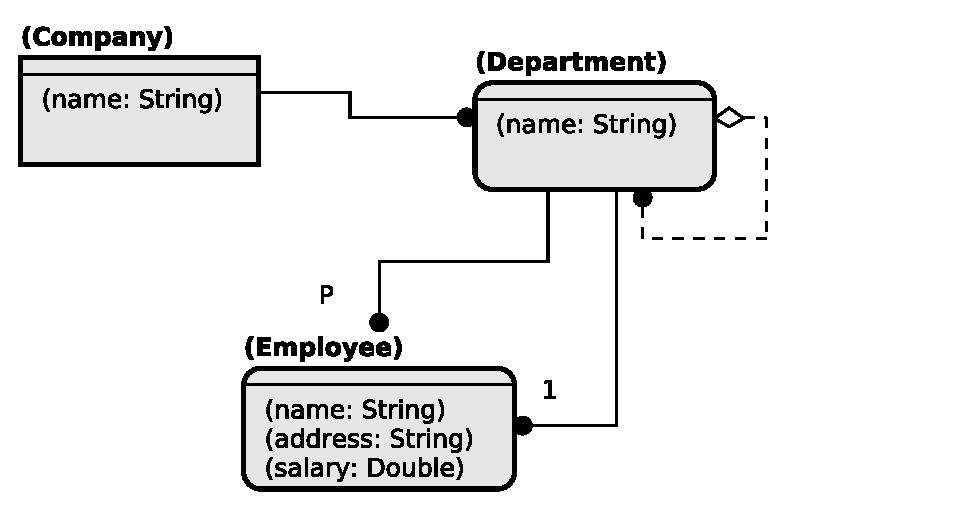
\includegraphics[width=\textwidth]{images/er-companies.pdf}
\caption{Diagrama UML para ilustração do modelo adaptado de \cite{favre2012101companies}}
\label{figura:tela do questionario}
\end{figure}


\subsection{\textit{Annonymous Inner Classes} e \textit{Expressões lambda}} 

 Antes das \emph{expressão Lambda} serem suportadas em Java, era necessário declarar uma \emph{Classe Interna Anônima} para passar um método (comportamento) como parâmetro para outro método. Este método permite que classes anônimas sejam definidas e instanciadas. Este método implementa o método de interface existente. Embora seja fácil implementar classes anônimas, esse recurso  pode ser visto como redundante e afetar a legibilidade e compreensão do seu código por outros desenvolvedores~\cite{tavares2017caracterizando}. A Listagem~\ref{anonima1} a seguir, ilustra como fazer a comparação de dois funcionários da empresa. A classe anônima instância o método de uma interface funcional que faz a comparação entre dois funcionários. A solução tradicional faz a verificação se os funcionários são iguais e caso a condição seja atendida é retornado um \emph{booleano true}.

 \newpage

\begin{lstlisting}[caption={Solução tradicional utilizando classe anônima},label={anonima1},captionpos=t]
Compare verify = new Compare() {
	@Override
	public boolean compareEmployees(Employee e1, Employee e2) {
		if (e1.equals(e2)) {
			return true;
		}
		return false;
	}
};
\end{lstlisting}

A Listagem~\ref{anoniTolambda} ilustra o código correspondente utilizando \emph{expressão lambda}. Podemos observar que a quantidade de linhas necessárias para realizar essa operação teve uma redução significativa.

\begin{lstlisting}[caption={Solução utilizando expressão lambda},label={anoniTolambda},captionpos=t]
Compare verify = (e1, e2) -> e1.equals(e2);
\end{lstlisting}

A seção a seguir é um exercicio onde aplicamos transformações de código para rejuvenescer programas em Java.

\section{Exercícios}

Vamos criar as classes do sistema com base no Diagrama UML acima~\ref{der-companies} e vamos implementar duas operações. Primeiro, vamos implementar uma operação de 
corte de salários em um departamento (e seus sub-departamentos). Em seguida, vamos calcular o total de salários em um departamento (e seus sub-departamentos). As operações devem ser nomeadas como \emph{cutSalaries(...); e totalSalary(...)} respectivamente. Além disso, devemos criar as operações utilizando recursos como $For \; loops$ tradicionais.

Abra o IntelliJ IDEA e selecione "New Project". Selecione "Java" no painel esquerdo e escolha a versão 8 do Java. Certifique-se de que "Create project from template" está desmarcado e clique em "Next".

Na próxima tela, escolha um nome para o seu projeto e selecione um local onde deseja salvá-lo. Clique em "Finish" para criar o projeto. Clique com o botão direito do mouse no diretório do seu projeto e selecione "New" e, em seguida, "Java Class". Dê um nome à sua classe e clique em "OK". Copie o código das classes e da interface funcional a seguir:

\newpage 

\begin{lstlisting}[caption={Classe Employee},label={anoniTolambda},captionpos=t]
package pt.uminho.companies;

public class Employee implements Unit{
	private String name; 
	private double salary;
	private double bonus;
	private String office;
	private Department department;
	
	public Employee(String name, double salary, double bonus, String office, Department department) {
		this.name = name;
		this.salary = salary;
		this.bonus = bonus;
		this.office = office;
		this.department = department;
	}

	public String getName() {
		return name;
	}

	public double getSalary() {
		return salary;
	}

	public double getBonus() {
		return bonus;
	}
		
	public String getOffice() {
		return office;
	}
	
	public Department getDepartment() {
		return department;
	}
        
        \\ Criar operacao cutSalaries()
        \\ Criar operacao totalSalary()
}
\end{lstlisting}

\newpage

\begin{lstlisting}[caption={Classe Department},label={anoniTolambda},captionpos=t]

package pt.uminho.companies;

import java.util.ArrayList;
import java.util.List;
import java.util.stream.Collectors;

public class Department implements Unit {

	private String name;
	private List<Department> subdepts;
	private List<Employee> employees;
	private Company company;

	public Department(String name, Company company) {
		this.name = name;
		this.company = company;
		subdepts = new ArrayList<>();
		employees = new ArrayList<>();
	}

	public void addDepartment(Department d) {
		subdepts.add(d);
	}

	public void addEmployee(Employee e) {
		employees.add(e);
	}

	public List<Employee> getEmployees() {
		return employees;
	}

        \\ Criar operacao cutSalaries()
        \\ Criar operacao totalSalary()
}
\end{lstlisting}

\newpage

\begin{lstlisting}[caption={Classe Company},label={anoniTolambda},captionpos=t]
package pt.uminho.companies;

import java.util.ArrayList;
import java.util.List;
import java.util.stream.Collector;
import java.util.stream.Collectors;

public class Company implements Unit {

	private String name;
	private List<Department> departments;

	public Company(String name) {
		this.name = name;
		this.departments = new ArrayList<>();
	}

	public String getName() {
		return name;
	}

	public List<Department> getDepartments() {
		return departments;
	}

	public void addDepartment(Department d) {
		departments.add(d);
	}

        \\ Criar operacao cutSalaries()
        \\ Criar operacao totalSalary()
 }
\end{lstlisting}

\begin{lstlisting}[caption={Interface Unit},label={anoniTolambda},captionpos=t]
package pt.uminho.companies;

public interface Unit {
	
	public void cutSalaries(double percent);
	public double totalSalary();

}
\end{lstlisting}


Vamos criar também a suite de testes que vão validar as implementações das operações e o nosso sistema. Abra o explorador de arquivos e navegue até o diretório raiz do projeto Java que você criou. Crie uma nova pasta com o nome "test" ou "tests". Esta pasta será o local onde você armazenará seus arquivos de teste.

Para criar testes automatizados em Java, você precisará adicionar uma biblioteca de teste ao seu projeto. Existem várias bibliotecas de teste disponíveis, mas uma das mais populares é o JUnit. Para adicionar o JUnit ao seu projeto no IntelliJ IDEA, siga os seguintes passos:

\begin{itemize}
    \item Clique com o botão direito do mouse no diretório do projeto e selecione "Open Module Settings".
    \item Selecione a guia "Dependencies".
    \item Clique no botão "+" e selecione "Library".
    \item Selecione "JUnit" na lista de bibliotecas disponíveis e clique em "OK".
\end{itemize}

Clique com o botão direito do mouse na pasta "test" que você criou e selecione "New" e, em seguida, "Java Class". Dê um nome à sua classe de teste e certifique-se de que ela esteja no pacote correto. Por convenção, os nomes das classes de teste devem terminar com "Test". Adicione ao seu programa os testes abaixo:


\begin{lstlisting}[caption={Classe EmployeeTest},label={anoniTolambda},captionpos=t]
package pt.uminho.companies;

import org.junit.jupiter.api.Test;

import static junit.framework.Assert.assertEquals;
import static junit.framework.Assert.assertTrue;

class EmployeeTest {

	@Test
	public void testCutSalary() {
		Company com = new Company("Universidade do Minho");
		Department dep = new Department("Haslab", com);
		Employee emp = new Employee("Joao Saraiva", 100.0, 20.0, "manager", dep);

		assertEquals(120.0, emp.totalSalary(), 0.01);

		emp.cutSalaries(5.0);

		assertEquals(115.0, emp.totalSalary(), 0.01);
	}

	@Test
	public void testCutSalaries() {
		Company com = new Company("Universidade do Minho");
		Department dep = new Department("Haslab", com);
		Employee emp = new Employee("Joao Saraiva", 100.0, 20.0, "manager", dep);

		emp.cutSalaries(5.0);

		assertEquals(115.0, emp.totalSalary(), 0.01);
	}

 }

\end{lstlisting}

\newpage

\begin{lstlisting}[caption={Classe DepartmentTest},label={anoniTolambda},captionpos=t]
package pt.uminho.companies;

import static org.junit.jupiter.api.Assertions.assertEquals;
import org.junit.jupiter.api.Test;

public class DepartmentTest {

	@Test
	public void testTotalSalary() {

		Company com = new Company("Universidade do Minho");
		Department dep1 = new Department("Haslab", com);
		Department dep2 = new Department("INESC", com);
		Employee emp = new Employee("Rodrigo", 10000.0, 500.0, "manager", dep2);
		Employee emp2 = new Employee("Walter", 100.0, 20.0, "developer", dep2);
		Employee emp3 = new Employee("Joao Saraiva", 5000.0, 200.0, "developer", dep2);

		com.addDepartment(dep1);
		com.addDepartment(dep2);

		dep2.addEmployee(emp);
		dep2.addEmployee(emp2);
		dep2.addEmployee(emp3);

		assertEquals(15820.0, dep2.totalSalary(), 0.01);
	}

	@Test
	public void testCutSalaries() {

		Company com = new Company("Universidade do Minho");
		Department dep1 = new Department("Haslab", com);
		Department dep2 = new Department("INESC", com);
		Employee emp = new Employee("Rodrigo", 10000.0, 500.0, "manager", dep2);
		Employee emp2 = new Employee("Walter", 100.0, 20.0, "developer", dep2);
		Employee emp3 = new Employee("Joao Saraiva", 5000.0, 200.0, "developer", dep2);

		com.addDepartment(dep1);
		com.addDepartment(dep2);

		dep2.addEmployee(emp);
		dep2.addEmployee(emp2);
		dep2.addEmployee(emp3);

		dep2.cutSalaries(10.0);

		assertEquals(14310.0, dep2.totalSalary(), 0.01);
	}
}

\end{lstlisting}


\begin{lstlisting}[caption={Classe CompanyTest},label={anoniTolambda},captionpos=t]
package pt.uminho.companies;

import static org.junit.jupiter.api.Assertions.assertEquals;
import org.junit.jupiter.api.Test;

public class CompanyTest {
	
	@Test
	public void testCutSalaries() {
		Company com = new Company("Universidade do Minho");
		Department dep1 = new Department("Haslab", com);
		Department dep2 = new Department("INESC", com);
		Employee emp = new Employee("Rodrigo", 5000.0, 900.0, "manager", dep2);
		Employee emp2 = new Employee("Walter", 100.0, 20.0, "developer", dep2);
		Employee emp3 = new Employee("Joao Saraiva", 2000.0, 200.0, "developer", dep2);
		
		com.addDepartment(dep1);
		com.addDepartment(dep2);
		
		dep2.addEmployee(emp);
		dep2.addEmployee(emp2);
		dep2.addEmployee(emp3);
		
		dep2.cutSalaries(10.0);

		assertEquals(7510.0, dep2.totalSalary(), 0.01);
	}
	
	@Test
	public void testTotalSalary() {
		Company com = new Company("Universidade do Minho");
		Department dep1 = new Department("Haslab", com);
		Department dep2 = new Department("INESC", com);
		Employee emp = new Employee("Rodrigo", 5000.0, 900.0, "manager", dep2);
		Employee emp2 = new Employee("Walter", 100.0, 20.0, "developer", dep2);
		Employee emp3 = new Employee("Joao Saraiva", 2000.0, 200.0, "developer", dep2);
		
		com.addDepartment(dep1);
		com.addDepartment(dep2);
		
		dep2.addEmployee(emp);
		dep2.addEmployee(emp2);
		dep2.addEmployee(emp3);
		
		assertEquals(8220.0, dep2.totalSalary(), 0.01);
	}
}

\end{lstlisting}

Após implementar as operações, vamos validar se todos os testes estão passando. Para executar os testes, clique com o botão direito do mouse na classe de teste que você criou e selecione "Run 'testName'". O IntelliJ IDEA executará todos os testes na classe de teste e mostrará o resultado no console. 



%Sets the bibliography style to UNSRT and imports the 
%bibliography file "sample.bib".
\bibliographystyle{unsrt}
\bibliography{bibliografia}



\end{document}
